\chapter{Koma Higikorreko Aritmetika.}
\label{sec:4}

\section{Sarrera.}

Konputagailuetan, zenbaki errealak ($\mathbb{R}$) bit kopuru finituaren bidez adierazi behar dira eta honetarako, koma-higikorreko adierazpen sistema ($\mathbb{F}$) erabiltzen da. Zenbaki erreal batzuk, $\mathbb{F}$ sisteman adierazpen zehatza dute, baina beste batzuk hurbildu egin behar dira.  Era berean, eragiketa aritmetikoen ($+,-,*,/$) kalkulu gehienetan ere, emaitzaren hurbilpena egin beha da. $\mathbb{R}$ sistematik $\mathbb{F}$ sistemara bihurtzeko funtzioari biribiltzea esaten zaio. Oro har konputazio zientzietan, biribiltze errore honen eragina garrantzitsua da eta errorea gutxitzeko ahalegin berezia beharrezkoa da.

Egungo konputagailuen koma-higikorreko aritmetikaren inplementazioak, \emph{IEEE $754$} estandarrean oinarritzen dira. 
\emph{IEEE-$754$} estandarrak, koma-higikorreko aritmetikaren konputaziorako formato eta metodoak definitzen ditu. Konputazioen fidagarritasuna eta aplikazioen portabilitatea bermatzen ditu.    
 
Atal honetan, koma-higikorreko aritmetikaren oinarria eta biribiltze errorea azalduko ditugu. Ondoren, konputazioetan biribiltze erroreak gutxitzeko teknika ezagun batzuk azalduko ditugu. 

\section{\emph{IEEE-754} estandarra.}

Koma-higikorreko zenbaki multzoa finitua da eta ${\mathbb{F}}$ izendatuko dugu. Koma-higikorreko adierazpen zehatza duten zenbaki errealei koma-higikorreko zenbakiak deritzogu, 
\begin{equation*}
\mathbb{F}\subset \mathbb{R}.
\end{equation*}

\paragraph*{}$\mathbb{F}$ zenbaki multzoa (Irudia \ref{fig:FloatNumberLine} Irudia) irudian laburtu dugu. Bai zenbaki positiboentzat, bai negatiboentzat, adierazi daitekeen zenbaki handienaren eta txikienaren arteko balio bakanez osatuta dago. Multzoaren kanpoaldean zenbaki hauek guztiak ditugu: batetik overflow tartean $(-\infty,\max_{x \in \mathbb{F_{-}}}|x|)$  eta $(\max_{x \in \mathbb{F_{+}}}|x|,\infty+)$ daudenak; bestetik underflow tartean  $(\min_{x \in \mathbb{F_{-}}}|x|,0)$ eta $(0,\min_{x \in \mathbb{F_{+}}}|x|)$ daudenak. 

\begin{figure}[h]
\centerline{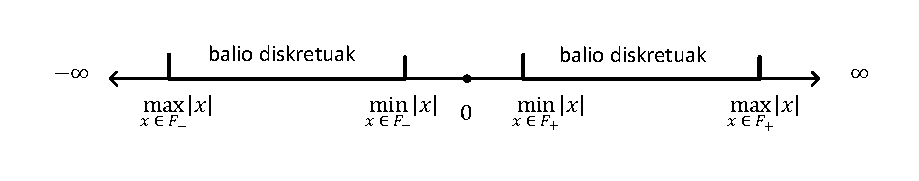
\includegraphics[width=14cm, height=3cm] {ZenbakiErrealak}}
\caption{Koma-higikorreko zenbakien adierazpena.}
\label{fig:FloatNumberLine}
\end{figure} 

IEEE-754 estandarraren arabera, $n$-biteko koma-higikorreko adierazpenak bi zati ditu (ikus \ref{fig:32bitKomaHigikorra} irudiko adibidea),
\begin{enumerate}
\item $m$ bitez osatutako zatia, mantisa izenekoa eta $M$ zenbaki erreala adierazten duena. Horietako bit bat ($S$) zeinua adierazten du. Bestalde $M$ mantisa modu normalizatu honetan emana da, $\pm 1.F$ eta zati erreala ($F$) bakarrik gordetzen da.   
\item Esponentea ($E$), $(n-m)$ bitez adierazitako zenbaki osoa. Zeinuarentzat ez da bit zehatzik, baizik \emph{bias} izeneko balio bat gehituz adierazten dira zenbaki positiboak eta negatiboak.  
\end{enumerate}

Beraz, oinarri bitarrean koma-higikorreko zenbaki hauek adierazten dira,
\begin{equation*}
M \times b^E, \ b=2,
\end{equation*}
eta biribiltze unitatea (\emph{unit roundoff}) era honetan definituko dugu,
\begin{equation*}
u=2^{-m}.
\end{equation*} 

\begin{figure}[h]
\centerline{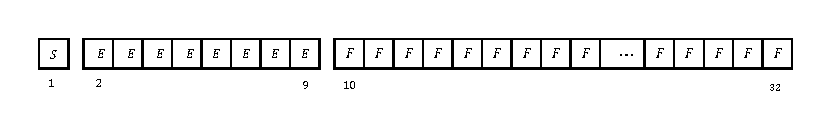
\includegraphics[width=12cm, height=2cm] {ZenbakiErrealak2}}
\caption[32-biteko koma-higikorra]{\small $32$-biteko koma-higikorreko zenbakiaren adierazpena: esponentearentzat  8-bit eta mantisarentzat  $24$-bit (bit bat zeinuarentzat eta beste $23$ bit, $1.F$ eran normalizatutako mantisarentzat) banatuta.}
\label{fig:32bitKomaHigikorra}
\end{figure} 

IEEE-$754$ estandarrean, oinarri bitarreko koma-higikorreko hiru formato definitzen dira: bata doitasun arrunta (\emph{single precision}), bestea doitasun bikoitza (\emph{double precision}) eta hirugarrena doitasun laukoitza (\emph{quadruple precision}) izenekoak (\ref{tab:koma-higikorreko-aritmetikak} Taula).

\begin{table} [h!]
\caption{}
\label{tab:koma-higikorreko-aritmetikak}       % Give a unique label
\centering
\begin{tabular}{ l c c c l c} 
 \hline
 Formatoa      &  Tamaina    & m   & e  & Tartea           &  $u=2^{-m}$          \\
   \hline
% Half     & 16 bit      & 11  & 5  & $2^{\pm 16}$     &  $5 \times 10^{-4}$   \\ 
 Arrunta   & 32 bit      & 24  & 8  & $10^{\pm 38}$    &  $6 \times 10^{-8}$   \\	    
 Bikoitza  & 64 bit      & 53  & 11 & $10^{\pm 308}$   &  $1 \times 10^{-16}$   \\
 Laukoitza & 128 bit     & 113 & 15 & $10^{\pm 11356}$ &  $1 \times 10^{-35}$   \\
\hline
\end{tabular}
\end{table}


Doitasun bikoitzeko oinarrizko eragiketak (batuketa, kenketa, biderketa, zatiketa, eta erro karratua) hardware bidez exekutatzen dira \cite{Muller2009} eta azkarrak dira. Makina ziklo bakoitzeko, $2$ eta $4$ batuketa, kenketa edo biderketa egin ohi dira; zatiketa eta erro karratua aldiz eragiketa motelagoak dira. Bestalde, doitasun arruntaren  aritmetika, doitasun bikoitza baino azkarragoa da: garraiatu behar den bit kopuru erdia delako eta gainera, hardware bereziei (\emph{Intel} makinetan \emph{SSE} moduloak) esker,  eragiketa aritmetikoak azkarragoak direlako. 2008. urtean, IEEE-$754$ estandarrak $128$-biteko koma-higikorreko aritmetika onartu zuen bainan bere inplementazioa  softwarez bidezkoa da eta exekuzioa gutxi gorabehera doitasun bikoitzeko aritmetika baino 10-15 aldiz motelagoa da.

\paragraph*{} Problema batzuk, doitasun bikoitza bainon doitasun handiagoa behar dute \cite{Joldes2016}. Doitasun laukoitza edo altuagoa, software liburutegien bidez emulatzen ohi dira. Doitasun altuko zenbakiak adierazteko nagusiki bi modu bereizten dira:   

\begin{enumerate}
\item \emph{Digito-anitzeko adierazpena}. Zenbakiak exponente bakarra eta mantisa bat baino gehiagorekin adierazten dira (adbz \emph{GNU MPFR liburutegia}).
\item \emph{Termino-anitzeko adierazpena}. Zenbakiak  ebaluatu gabeko hainbat koma-higikorreko makina zenbaki estadarren batura gisa adierazten dira (adbz Bailey QD liburutegia) eta exekuzioaren ikuspegitik, hardware bidezko inplementazioaren abantaila dute.    
\end{enumerate}

\emph{GCC libquadmath} liburutegia erabili dugu doitasun laukoitzeko gure esperimentuetarako. Doitasun laukoitzeko integrazioak, soluzio zehatzak kontsideratu ditugu eta  doitasun bikoitzeko inplementazioaren errorea, soluzio zehatzaren diferentzi gisa kalkulatu dugu. 

Laskar-ek epe luzeko eguzki-sistemaren simulazioaren ($-250$ eta $+250$ milioitako integrazio tartea) konputaziorako kalkuluak, kontu handiz eta doitasun handian egin behar ditu. Dena den, era honetako problemak salbuezpenak dira. Ez da ohikoa izaten doitasun handian lan egin beharra eta egia da ere, neurri fisiko oso gutxi ezagutzen direla  hain doitasun handian (adibidez $50$-bitekin, lurra eta ilargiaren arteko distantzia bakteria baten neurriaren  bainon errorea txikiagoarekin adierazi daiteke).  


\section{Biribiltze errorea.}

Zenbakizko integrazioen errorea, trunkatze eta biribiltze errorez osatuta dago. Urrats luzera adina txikia aukeratuz, trunkatze errorea biribiltze errorea baino txikiago izango da eta beraz, zenbakizko integrazioaren errorean biribiltze errorea nagusitzen da. Epe luzeko eta doitasun handiko integrazioetan urrats luzera txikia erabiltzen denez, biribiltze errorea gutxitzea funtsezkoa izango da.     

Bi biribiltze mota bereiziko ditugu, bata adierazpen errorea eta beste eragiketa (aritmetika) errorea.  

\subsection*{Adierazpen errorea.} 

Zenbaki erreal batzuk, $\mathbb{F}$ koma-higikorreko multzoan zehazki adieraz daitezke eta beste batzuk ordea, hurbilpen batez adierazi behar dira. $x \in \mathbb{R}$ izanik, $fl: \mathbb{R} \rightarrow \mathbb{F}$ koma-higikorreko zenbakia esleitzen dion funtzioari deituko diogu. $fl(x)$, $\mathbb{F}$ multzoan $x$-en gertuen dagoen balioa bezala definitzen da.   

Jarraian, koma-higikorreko adierazpenaren errore absolutua eta errore erlatiboa finkatuko ditugu.
\begin{itemize}
\item Errore absolutua,
\begin{equation*}
\triangle x= fl(x)-x= \tilde{x}-x. 
\end{equation*} 
\item Errore erlatiboa, 
\begin{equation*}
\delta x =\frac{\triangle x}{x} = \frac{\tilde{x}-x}{x}. 
\end{equation*}
\item Aurreko bi definizioen ondorioz honako formula erabilgarria dugu,
\begin{equation*}
\tilde{x}= x+\triangle x = x \ (1+\delta x).
\end{equation*}
\end{itemize}

Koma-higikorreko zenbaki sistema bitarrean ($m=$ mantisa adierazteko bit kopurua izanik) $|x|$ balioa, $\mathbb{F}$ multzoaren zenbaki txikienaren eta handienaren artean badago,
\begin{equation*}
 |\delta x|< u \ \ \text{non} \ \ u=2^{-m},
 \end{equation*}
bermatuta dagoela frogatu daiteke.

\subsection*{Eragiketen errorea.} 

Koma-higikorreko zenbakien arteko eragiketa baten emaitzak ez du $\mathbb{F}$ multzoan adierazpen zehatza izan behar eta emaitzaren hurbilpena kontsideratuko da. Adibidez, orokorrean $m$ digituzko bi mantisen biderketaren emaitza zehatza adierazteko, $2m$ digituzko mantisa behar dugu ($m$ digituzko galera) \cite{Fukushima2001}. Salbuespena, biderkagaietako bat $2$ren berredura denean gertatzen da, orduan biderketa zehatza baita.

\paragraph*{Adibidea.} Demagun hiru digitu hamartar errealeko aritmetikarekin ari garela lanean.

Emaitza zehatza, $1,343 \times 2,103 = 2,824229$. 

Hiru digitu hamartar errealeko aritmetika, $1,343 \times 2,103 \approx 2.824$.

\paragraph*{} Hauek zenbaki errealen arteko funtsezko eragiketak badira,  $\ast: \mathbb{R}^2\rightarrow \mathbb{R}$, 
\begin{equation*}
\ast\in \{+,-,\times,/ \},
\end{equation*}
koma-higikorreko zenbakien arteko funtsezko eragiketak era honetan izendatuko ditugu  $\circledast: \mathbb{F}^2\rightarrow \mathbb{F}$,
\begin{equation*}
\circledast\in \{\oplus,\ominus,\otimes,\oslash \}.
\end{equation*}

$\tilde x,\tilde y \in \mathbb{F}$ emanik eta $z= \tilde x \ast \tilde y$ emaitza zehatza bada, $\tilde z= \tilde x \circledast \tilde y$ (edo $\tilde z= fl(\tilde x \ast \tilde y$)) eragiketaren emaitzaren errore absolutua eta errore erlatiboa definituko ditugu,

\begin{itemize}
\item Errore absolutua,
\begin{equation*}
\triangle z=\tilde z-z =(\tilde x \circledast \tilde y) -(\tilde x \ast \tilde y).
\end{equation*} 
\item Errore erlatiboa,
\begin{equation*}
\delta z=\frac{\triangle z}{z}==\frac{(\tilde x \circledast \tilde y) -(\tilde x \ast \tilde y)}{(\tilde x \ast \tilde y)}.
\end{equation*} 
\item Honako erlazio hau ondorioztatu daiteke,
\begin{equation*}
\tilde z=(\tilde x \circledast \tilde y)=z+\triangle z=z \ (1+\delta z).  
\end{equation*}
\end{itemize}

Koma-higikorreko aritmetikan, \ $|\delta z|<u$ \ , non  $u=2^{-m}$, beteko dela frogatu daiteke.

\paragraph*{} Zenbakizko algoritmoen biribiltze errorearen eraginaren azterketak, propietate honetan oinarritzen dira. Bestalde, errore erlatiboak emaitzaren digitu zuzenak neurtzen du:
\begin{equation*}
\delta z \approx 10^{-k} \Rightarrow \ \approx \ k \ \mbox{digitu hamartar zuzen}.
\end{equation*}  


\subsection*{Biribiltze errorearen propagazioa.}


Ohiko konputazioetan, eragiketa aritmetiko kopuru handia egin behar dugu emaitza lortzeko. Batzuetan, eragiketa bakoitzaren biribiltze erroreak elkar ezereztatzen dira baina kasu txarrenean, biribiltze errorea metatu eta magnitude handikoa izan daiteke.   

\paragraph*{Adibidea.} 
Modu honetako batura batean , non $n>2$ eta $\tilde x_1,\dots,\tilde x_n \in \mathbb{F}$,  
\begin{equation*}
\bigoplus_{i=1}^{n}(\tilde x_i)=(\sum\limits_{i=1}^{n} \tilde x_i)(1+\delta),
\end{equation*}
ezin daiteke bermatu $|\delta|<u$ beteko denik. 

\paragraph*{}Analisi zehatza egiten badugu $n=3$ adibiderako, honako espresioa lortzen dugu,
\begin{equation*}
((\tilde x_1 \oplus \tilde x_2) \oplus \tilde x_3)  = 
  \big((\tilde x_1 + \tilde x_2)(1+\delta_1)
  +\tilde x_3 \big) (1+\delta_2), \ \ \delta_1,\delta_2<u.
\end{equation*}

\subsection*{Ezabapen arazoa.}

Algoritmoen kalkuluetan, doitasuna galera azkarra gerta daiteke. Horren adibidea ezabapen arazoa dugu: oso antzekoak diren bi zenbaki arteko kendura egiten dugunean gerta daitekeena. 

\paragraph*{Adibidea.}
\begin{lstlisting} [language=Mathematica]
>>  InputForm[N[Pi]]
>> 3.141592653589793

>> y=N[Pi]*10^(-10);
>> InputForm[y]
>> 3.1415926535897934*10^(-10)

>> z=1.+y;
>> InputForm[z]
>> 1.0000000003141594           # 16-digitu hamartar zuzenak.

>> InputForm[z-1.]
>> 3.141593651889707*10^(-10)   # 6-digitu hamartar zuzenak.

\end{lstlisting}


\section{Biribiltze errorearen gutxitzeko teknikak.}
\label{sec:4.4}

Batura eta biderketa eragiketen biribiltze errorearen konputaziorako algoritmoak ezagunak dira \cite{Dekker1971}\cite{Higham2002}. Algoritmo hauek, \emph{termino-anitzeko adierazpen} inplementazioetan erabiltzen dira eta baturaren kasuan, batura konpensatu izeneko algoritmoaren oinarria da. Ikusiko dugun bezala, algoritmo sinpleak dira eta konputazio kostu txikia dute.  

Ideia, teknika hauek zenbakizko integrazioaren inplementazioaren kalkulu "kritikoetan" erabiltzea da, soluzioaren doitasuna handitzeko asmoarekin.

\subsection*{Batura: Fast2Sum.}

\emph{Fast2Sum} algorithmoa, 1971an Dekker-ek \cite{Dekker1971} sortu zuen. Koma-higikorreko $\tilde x,\tilde y \in \mathbb{F} \ \text{non} \ |\tilde x| \geq |\tilde y|$ bi zenbakien, arteko baturari  $\tilde z= \tilde x \oplus \tilde y$,  dagokion biribiltze errorea $e , \ \text{non} \ \tilde z+ e=\tilde x+\tilde{y}$ den, era honetan kalkulatu daiteke,

\begin{algorithm}[H]
 \BlankLine
 {$\tilde{z}=\tilde{x} \oplus\tilde{y}$\;
  $e=\tilde{y} \ominus (\tilde{z}\ominus\tilde{x})$\;
 }
 \BlankLine
 \caption{Fast2Sum.}
 \label{alg:FastSum}
\end{algorithm}

\paragraph*{}Irudiaren (\ref{fig:fast2sum} Irudia) laguntzarekin hobeto uler daiteke baturaren biribiltze errorearen kalkulua.

\begin{figure}[h!]
\centerline{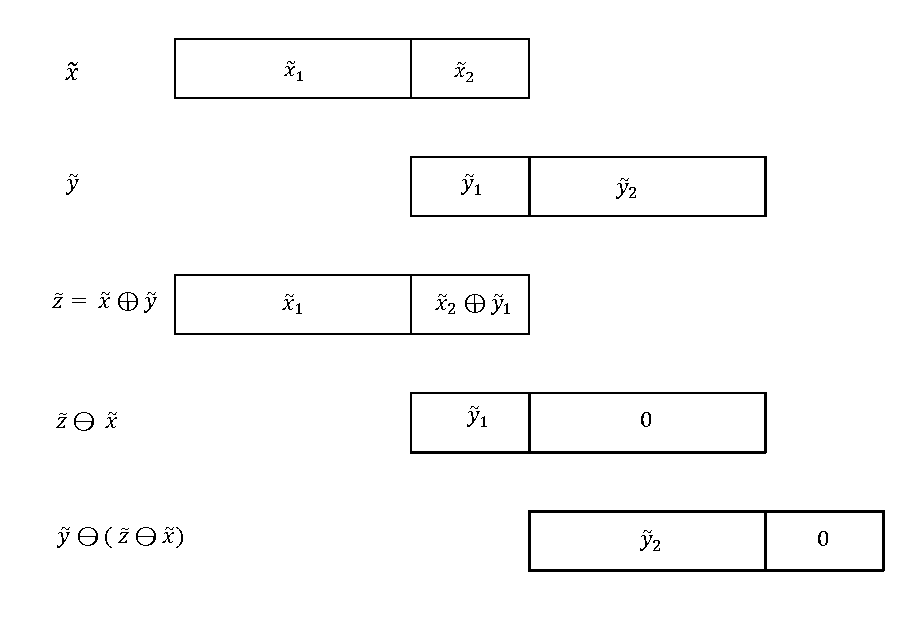
\includegraphics[width=12cm, height=6cm] {Fast2Sum}}
\caption{Batuketaren biribiltze errorea.}
\label{fig:fast2sum}
\end{figure} 

\subsubsection*{Batura konpensatua.}

Era honetako batura errekurtsiboetan,
\begin{equation*}
z_{n+1}= z_0+\sum\limits_{i=0}^{n} x_i,
\end{equation*}
biribiltze errorea gutxitzeko teknika ezaguna da \cite{Higham2002}.
Ideia da, bi zenbakien baturan egindako biribiltze errorea lortu, eta errore hau hurrengo baturan erabiltzea. Jarraian azaltzen den moduan, urrats bakoitzaren amaieran errore estimazioa ($e_{i}$) kalkulatuko dugu eta hurrengo urratsean, batugaiari gehituko diogu.

\begin{algorithm}[H]
 \BlankLine
  $\tilde z_0= z_0; \ e_0=0$\;
  \For{$i\leftarrow 0$ \KwTo $n$}
  {
   \BlankLine
    $x=\tilde z_i$\;
    $y= x_i+e_i$\;
    $\tilde z_{i+1}=x+y$\;
    $e_{i+1}=(x-z)+y$\;
   \BlankLine
  }
 \caption{Kahan-en batura konpensatua.}
   \label{alg:KahanBK}
\end{algorithm}

\paragraph*{}Knuth-ek eta Kahan-ek \cite{Muller2009},  batura konpensatuko algoritmoaren bidez kalkulatutako $z_{n+1}$ batura honakoa betetzen duela, 
\begin{equation*}
\left | z_{n+1} - (z_0+\sum_{i=0}^{n} x_i) \right | \leq (2u+ \mathcal{O}(nu^2)) \left(|z_0|+\sum_{i=1}^{n} |x_0|\right),
\end{equation*}
frogatu zuten.

\paragraph*{} Jakina, algoritmoaren gaiak bektoreak, $\tilde z_0, e_0, x_0, x_1, \dots, x_n \in \mathbb{F}^d$ diren kasurako orokortu daiteke. Beraz, \ref{alg:KahanBK} algoritmoa $n$ eta $d$ parametroak dituen funtzio familia gisa interpretatu daiteke,
\begin{equation*}
S_{n,d} : \mathbb{F}^{(n+3)d} \rightarrow \mathbb{F}^{2d},
\end{equation*}
zein $\tilde z_0, e_0, x_0, x_1, \dots, x_n \in \mathbb{F}^d$ argumentuak emanik, $\tilde z_{n+1}, e_{n+1} \in \mathbb{F}^d$ balioak itzultzen ditu, eta $\tilde z_{n+1}+e_{n+1}$, honako batura $\tilde z_0+e_0+x_0+x_1+ \dots+x_n$ adierazi nahi duen.
 

\paragraph*{} Zenbakizko integrazioetan, era honetako batura errekurtsiboa kalkulatu behar ditugu,
\begin{equation*}
y_{n+1}=y_n+\delta_n,
\end{equation*}  
non $|\delta_n|<|y_n|$ izan ohi da. Beraz, integrazioaren batura honen birbiltze errorea gutxitzeko, batura konpensatua erabiliko dugu.  

$y_{n+1} \in \mathbb{R}^{d},\quad y_{n+1}=\tilde y_{n}+\tilde \delta_n$ batura zehatza izanik eta $\tilde y_{n+1} \in \mathbb{F}^{d}, \quad \tilde y_{n+1}=\tilde y_{n} \oplus \tilde \delta_n$ koma-higikorreko hurbilpena izanik, batura konpensatuaren bidez lortutako errorearen estimazioa $e_{n+1}$ ,

\begin{algorithm}[H]
 \BlankLine
  $\tilde{y}_{0}=fl(y_{0}); \ e_0=fl(y_0-\tilde{y}_0)$\;
 \BlankLine
  \For{$n=1,2,\cdots \quad$}
  {
   \BlankLine
    $inc=\tilde {\delta}_n \oplus e_n$\;
    $\tilde {y}_{n+1}=\tilde{y}_n \oplus inc$\;
    $e_{n+1}=(\tilde{y}_n \ominus \tilde {y}_{n+1}) \oplus inc$\;
   \BlankLine
  }
 \caption{Batura konpensatua(zenbakizko integrazioa).}
\end{algorithm}

\paragraph*{}baturan egindako  biribiltze errore zehatza da,
\begin{equation}
y_{n+1}=\tilde {y}_{n+1}+e_{n+1}. 
\end{equation}

\paragraph*{}Goian aipatutako ideia,  beste ikuspegi batetik ere azaldu daiteke. Ikuspegi honen arabera, gure zenbakizko soluzioa, bi \emph{double} balioren bidez ($\tilde{y}_n,e_n$)  adierazten ari gara (ia doitasun laukoitza) eta beraz, interpretazio honen arabera, konputazio eragiketa batzuk ia doitasun laukoitzean egiten ariko ginateke. Zentzu honetan gure inplementazioan, hasierako balio zehatza $y_0=y(t_0)$, doitasun bikoitzeko bi zenbakiren bidez ($\tilde{y}_0, e_0$) hasieratuko dugu,
\begin{align*}
\tilde{y}_0 &=fl(y_0) ,\\
e_0 &=fl(y_0-\tilde{y}_0).
\end{align*}

\subsection*{Bidekerta: 2MultFMA.}

\emph{IEEE 754-2008} estandarrean, \emph{FMA} (\emph{fused multiply-add}) instrukzioa gehitu zen eta hurrengo urteetan, ordenagailu arruntetan zabaltzea espero da. Instrukzio honek, orokorrean konputazioak azkartzen ditu eta biderketa eskalarren, matrize biderkaduren eta polinomio ebaluazioen biribiltze errore txikitzen du. \emph{FMA} instrukzioa, zatiketa eta erro karratuaren algoritmo azkarren diseinuan ere erabiltzen da.


\emph{FMA} instrukzioak, era honetako konputazioetan biribiltze errore bakarra bermatzen du,
\begin{equation*}
fl(\tilde x \times \tilde y \pm \tilde z)= (\tilde x \times \tilde y\pm \tilde z) (1+\delta), \ \delta<u \ \ \text{non} \ \ u=2^{-m}.
\end{equation*}
 

\emph{FMA}  instrukzioa erabilgarri dagoenean, biderketaren biribiltze errorea kalkulatzea erraza da; $\tilde x,\tilde y \in \mathbb{F}$ bi zenbakien, arteko biderketari $\tilde z= fl(\tilde x \times \tilde y)$,  dagokion biribiltze errorea $e, \ \text{non} \  \tilde{z}+ e=\tilde x \times \tilde y$ den, era honetan kalkulatu daiteke,

\begin{algorithm}[H]
 \BlankLine
 {$\tilde{z}=fl(\tilde{x}\times\tilde{y})$\;
  $e=fl(\tilde{x}\times\tilde{y}- \tilde{z})$\;
 }
 \BlankLine
 \caption{2MultFMA.}
 \label{alg:2MultFMA}
\end{algorithm}

\subsection*{Sterbenz Teorema.}
Sterbenz teoremaren arabera \cite{Sterbenz1973}, bi zenbaki elkarrekiko  gertu daudenean, honako baldintza betetzen bada horien arteko kendura zehatza da.
\begin{equation}
\label{eq:4311}
x,y \in \mathbb{F}, \ \ \frac{y}{2}\leq x \leq 2y \ \ \ \Rightarrow \ \ \ x-y\in \mathbb{F}.
\end{equation}


\section{Laburpena.}

Koma-higikorreko aritmetikan sakontzeko honako bibliografia azpimarratuko dugu: Numerical computing with IEEE floating point arithmetic (Michael L.Overton) \cite{Overton2001}, Handbook of floating-point arithmetic (Jean-Michael Muller) \cite{Muller2009}, Accuracy and stability of numerical algorithms (Nicholas J Higham) \cite{Higham2002} eta A graduate introduction to numerical methods (Rober M Corless) \cite{Corless2013}.

